\documentclass[pdftex,12pt,a4paper]{article}

\usepackage{graphicx}  
\usepackage[margin=2.5cm]{geometry}
\usepackage{breakcites}
\usepackage{indentfirst}
\usepackage{pgfgantt}
\usepackage{pdflscape}
\usepackage{float}
\usepackage{epsfig}
\usepackage{epstopdf}
\usepackage[cmex10]{amsmath}
\usepackage{stfloats}
\usepackage{multirow}

\renewcommand{\refname}{REFERENCES}
\linespread{1.3}

\usepackage{mathtools}
%\newcommand{\HRule}{\rule{\linewidth}{0.5mm}}
\thispagestyle{empty}
\begin{document}
\begin{titlepage}
\begin{center}
\textbf{}\\
\textbf{\Large{ISTANBUL TECHNICAL UNIVERSITY}}\\
\vspace{0.5cm}
\textbf{\Large{COMPUTER ENGINEERING DEPARTMENT}}\\
\vspace{2cm}
\textbf{\Large{BLG 242E\\ DIGITAL CIRCUITS LABORATORY\\ EXPERIMENT REPORT}}\\
\vspace{2.8cm}
\begin{table}[ht]
\centering
\Large{
\begin{tabular}{lcl}
\textbf{EXPERIMENT NO}  & : & 1 \\
\textbf{EXPERIMENT DATE}  & : & 10.03.2023 \\
\textbf{LAB SESSION}  & : & FRIDAY - 14.00 \\
\textbf{GROUP NO}  & : & G08 \\
\end{tabular}}
\end{table}
\vspace{1cm}
\textbf{\Large{GROUP MEMBERS:}}\\
\begin{table}[ht]
\centering
\Large{
\begin{tabular}{rcl}
150200081  & : & KAAN KARATAŞ \\
150210719   & : & NACİ TOYGUN GÖRMÜŞ \\
\end{tabular}}
\end{table}
\vspace{2.8cm}
\textbf{\Large{SPRING 2023}}

\end{center}

\end{titlepage}

\thispagestyle{empty}
\addtocontents{toc}{\contentsline {section}{\numberline {}FRONT COVER}{}}
\addtocontents{toc}{\contentsline {section}{\numberline {}CONTENTS}{}}
\setcounter{tocdepth}{4}
\tableofcontents
\clearpage

\setcounter{page}{1}

\section{INTRODUCTION [10 points]}

The experiments and tests were conducted by making use of CADET, the function generator, and the oscilloscope. The primary objective of these experiments was to gain knowledge and proficiency in using CADET effectively. The experiments consisted of a total of six different activities.

\section{MATERIALS AND METHODS [40 points]}
Tools that was used on the experiments:
\begin{itemize}
    \item CADET
    \item 7404 Hex Inverter
    \item 7408 AND Gate
    \item 7432 OR Gate
    \item Oscilloscope
    \item Function Generator
\end{itemize}

\subsection{Part 1}
During this experiment, the specified expressions were transformed into logic circuits using electronic components such as the 7432 OR Gate, 7408 AND Gate, and 7404 Hex Inverter. These circuits were then configured and tested using CADET.

F1(a, b) = a + a · b

F2(a, b) = (a + b) · (a + b')
\begin{figure}[H]
	\centering
	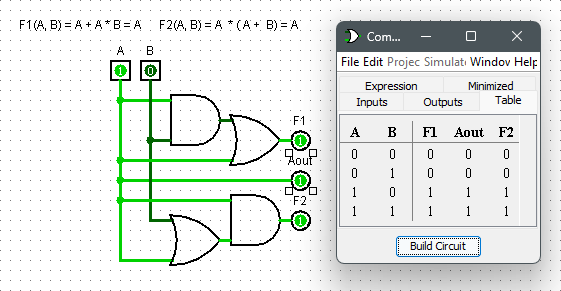
\includegraphics[width=0.7\textwidth]{ex1.png}	
	\caption{Diagram and Truth Table of F1 and F2}
	\label{fig1}
\end{figure}


Once we had finished constructing the circuits, we proceeded to verify their accuracy and ensure that they were functioning correctly.
\subsection{Part 2}
During this experiment, we designed a logic circuit on CADET using electronic components such as 7432 OR Gate and 7408 AND Gate. The circuit was created to represent the dual of the specified expression.

Expression: a + a · b = a

Expression's Dual: a . (a + b) = a
\begin{figure}[H]
	\centering
	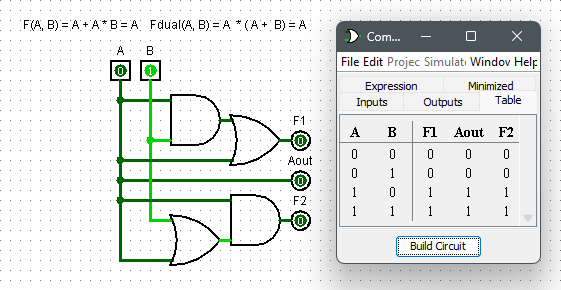
\includegraphics[width=0.9\textwidth]{ex2.png}
	\caption{Diagram and Truth Table of the Expression and  Expression's Dual}
	\label{fig2}
\end{figure}

After constructing the circuit that represented the dual expression, we proceeded to ensure that it was accurate. As expected, we verified that the dual expression was correct.
\subsection{Part 3}
During this experiment, we created logic circuits on CADET using electronic components such as the 7432 OR Gate, 7408 AND Gate, and 7404 Hex Inverter. These circuits were designed to represent both the complement of the specified expressions and the expression that realizes the complementary function.

Expression: F(a, b, c) = a · b + a' · c

Expression's Complement: F'(a, b, c) = (a · b + a' · c)'

Realized Function: F'(a, b, c) = (a' + b') . (a + c')

\begin{figure}[H]
	\centering
	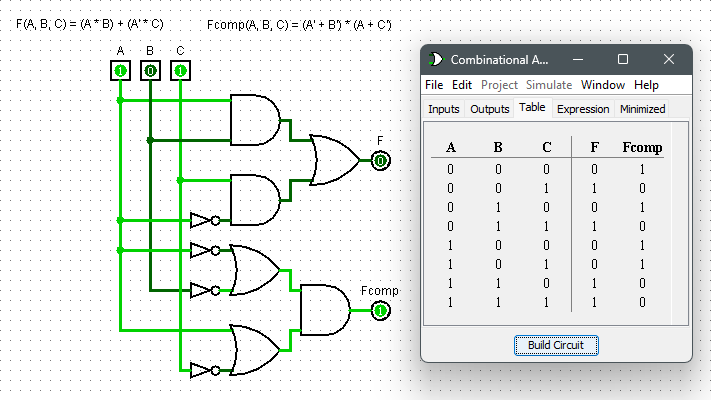
\includegraphics[width=0.9\textwidth]{ex3.png}
	\caption{Diagram and the truth table of the Expression and the Realized Expression}
	\label{fig3}
\end{figure}
Comparing the truth tables allowed us to validate the expression. Both truth tables were identical, as expected.

\subsection{Part 4}
In this experiment, following function's simplified form was implemented using logic gates.

F(a, b, c, d) = U(1, 2, 5, 6, 9, 10, 13, 14)

Simplifed F: (c . d') + (c' . d)

\begin{figure}[H]
	\centering
	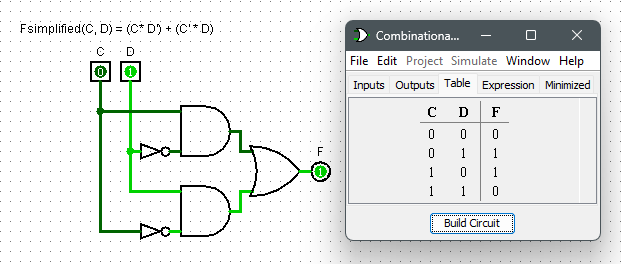
\includegraphics[width=1\textwidth]{ex4.png}
	\caption{Diagram and the Truth Table of the Simplified Form}
	\label{fig4}
\end{figure}



\subsection{Part 5}
\begin{itemize}
    \item In this section, a voltmeter was used to measure the Vcc and GND voltages.
    \begin{figure}[H]
	\centering
	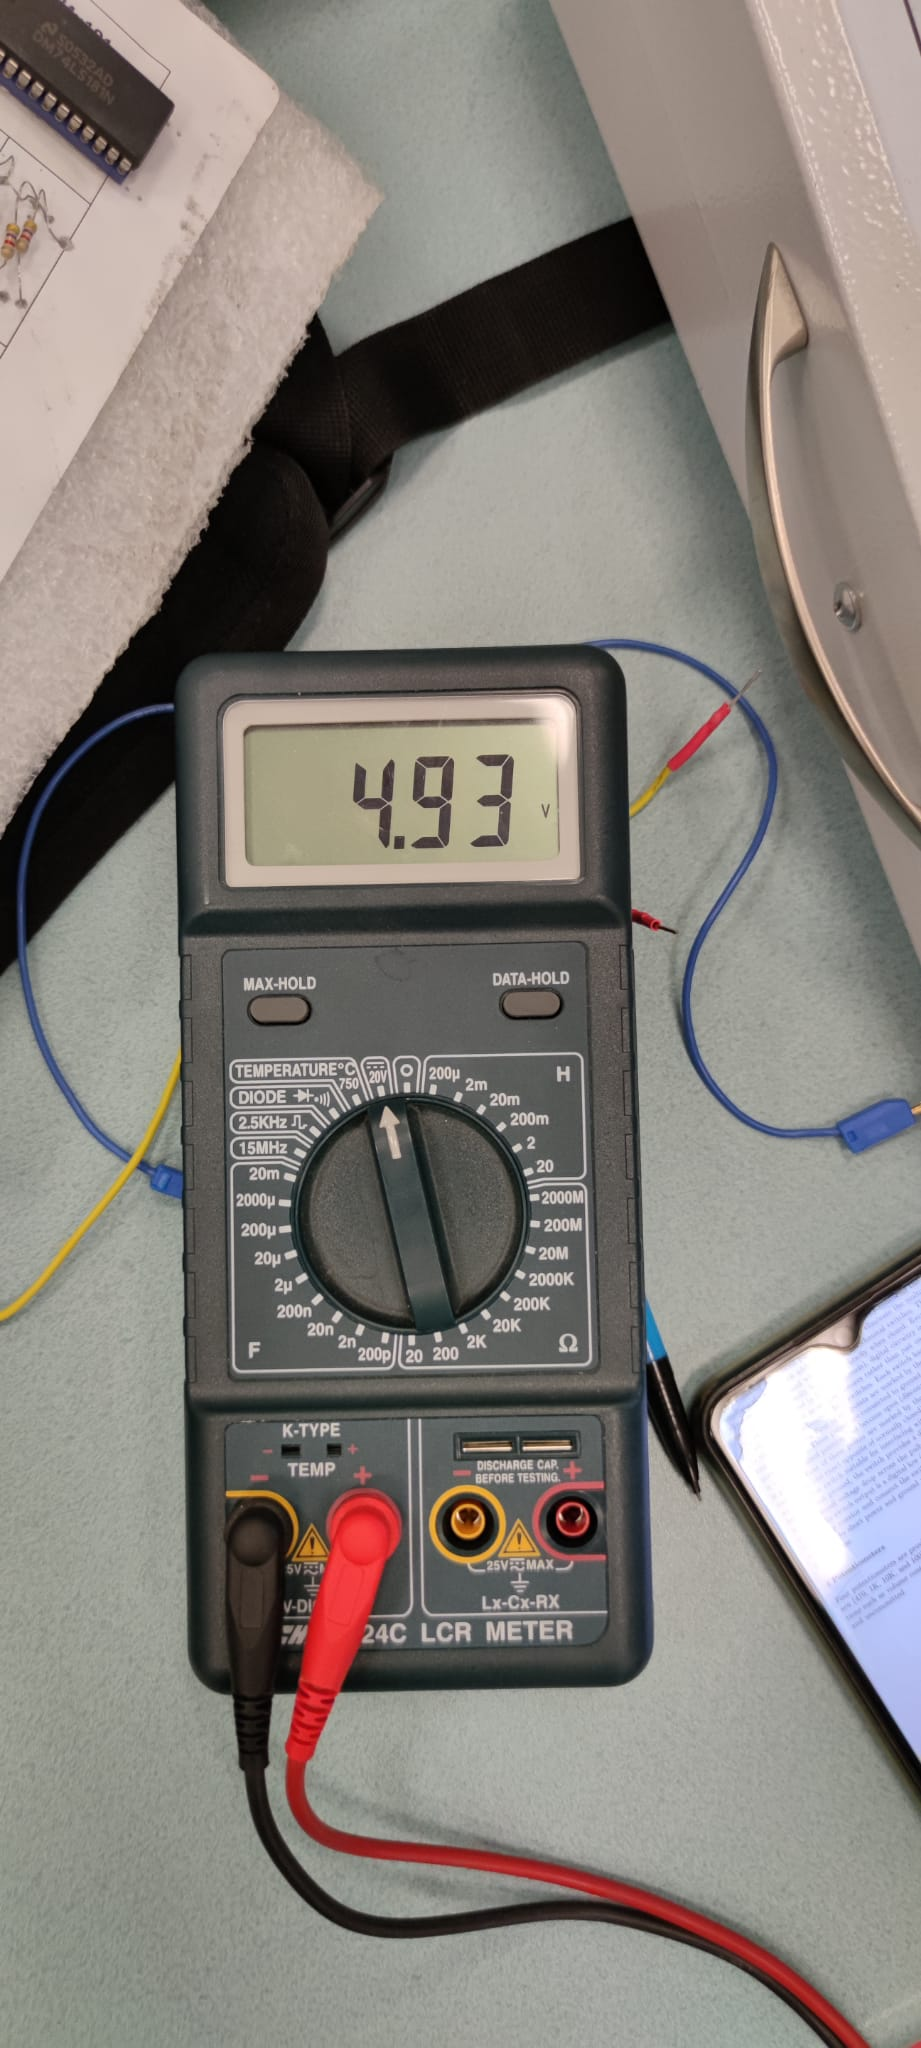
\includegraphics[width=0.5\textwidth]{ex5-1.png}
	\caption{5V Between Vcc GND}
	\label{fig5}
\end{figure}
    \vspace{4cm}
    \item In this section, an 8k Ohm resistor is built using a potentiometer.
    \begin{figure}[H]
	\centering
	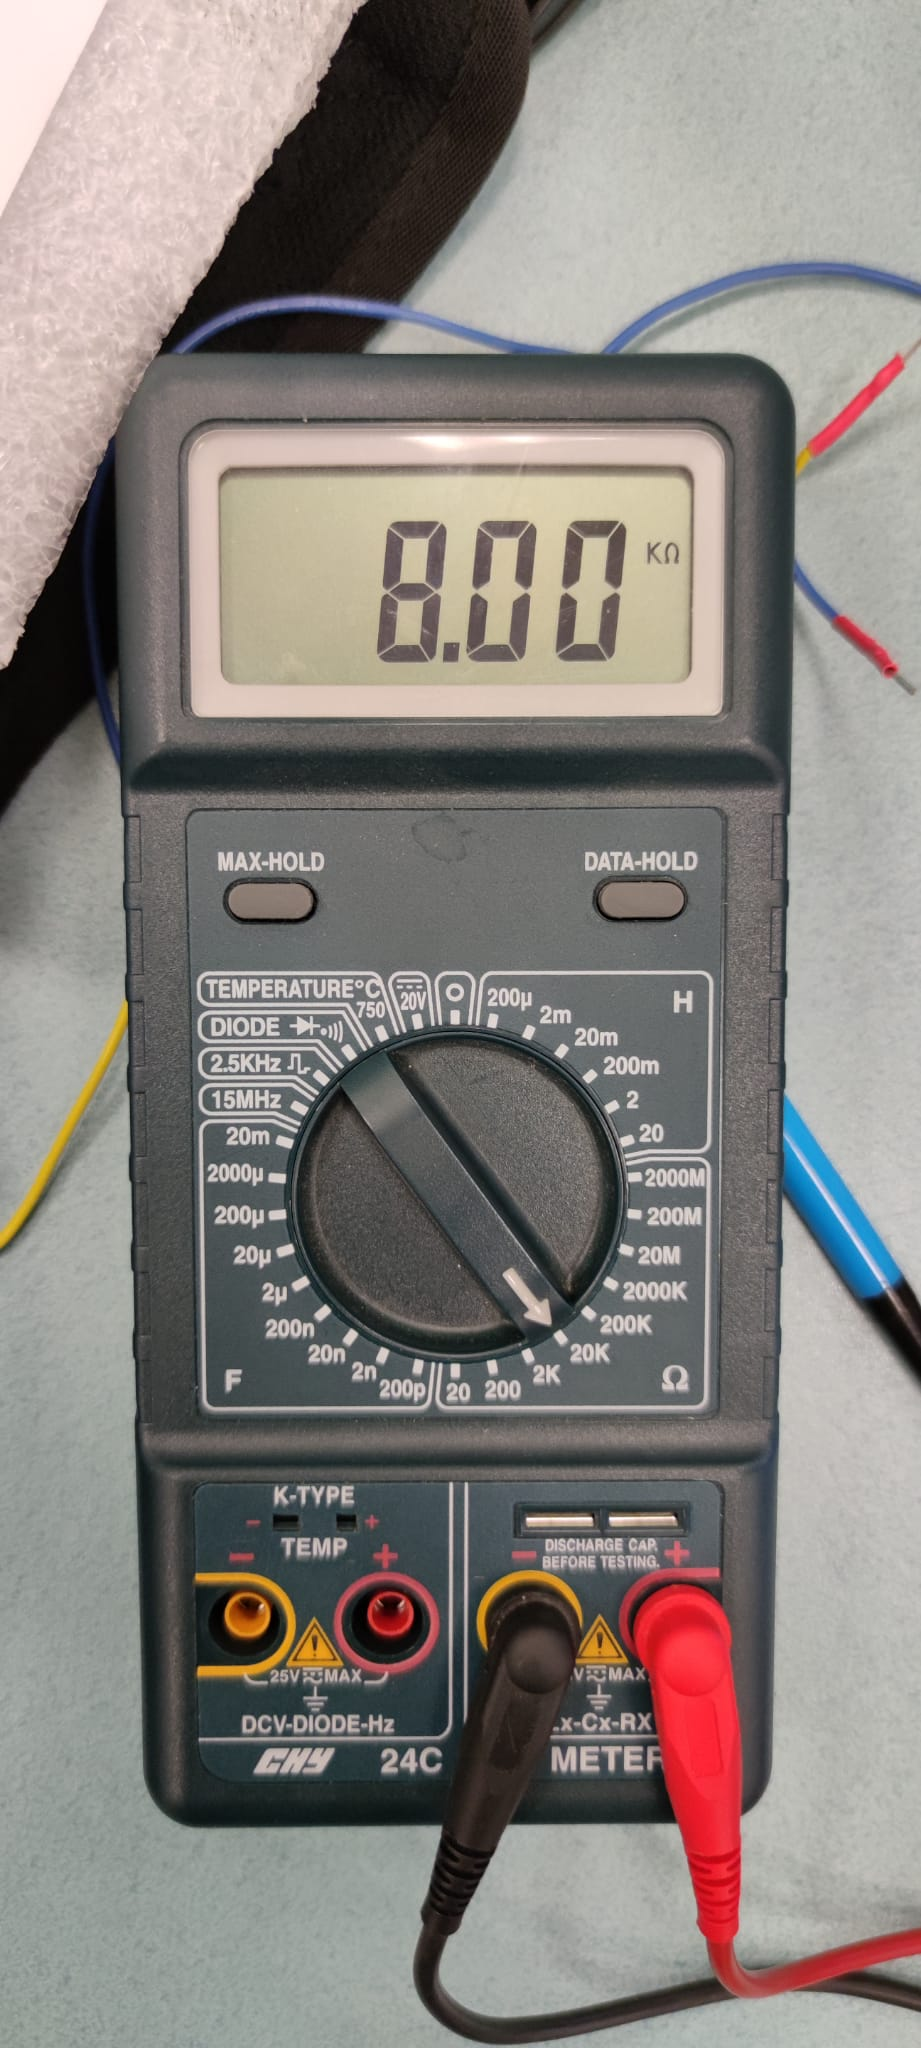
\includegraphics[width=0.5\textwidth]{ex5-2.png}
	\caption{8k Ohm Resistor}
	\label{fig6}
\end{figure}

    \item In this section, ”27” is showed in two seven segment display by giving an input using 8 switches.
    \begin{figure}[H]
	\centering
	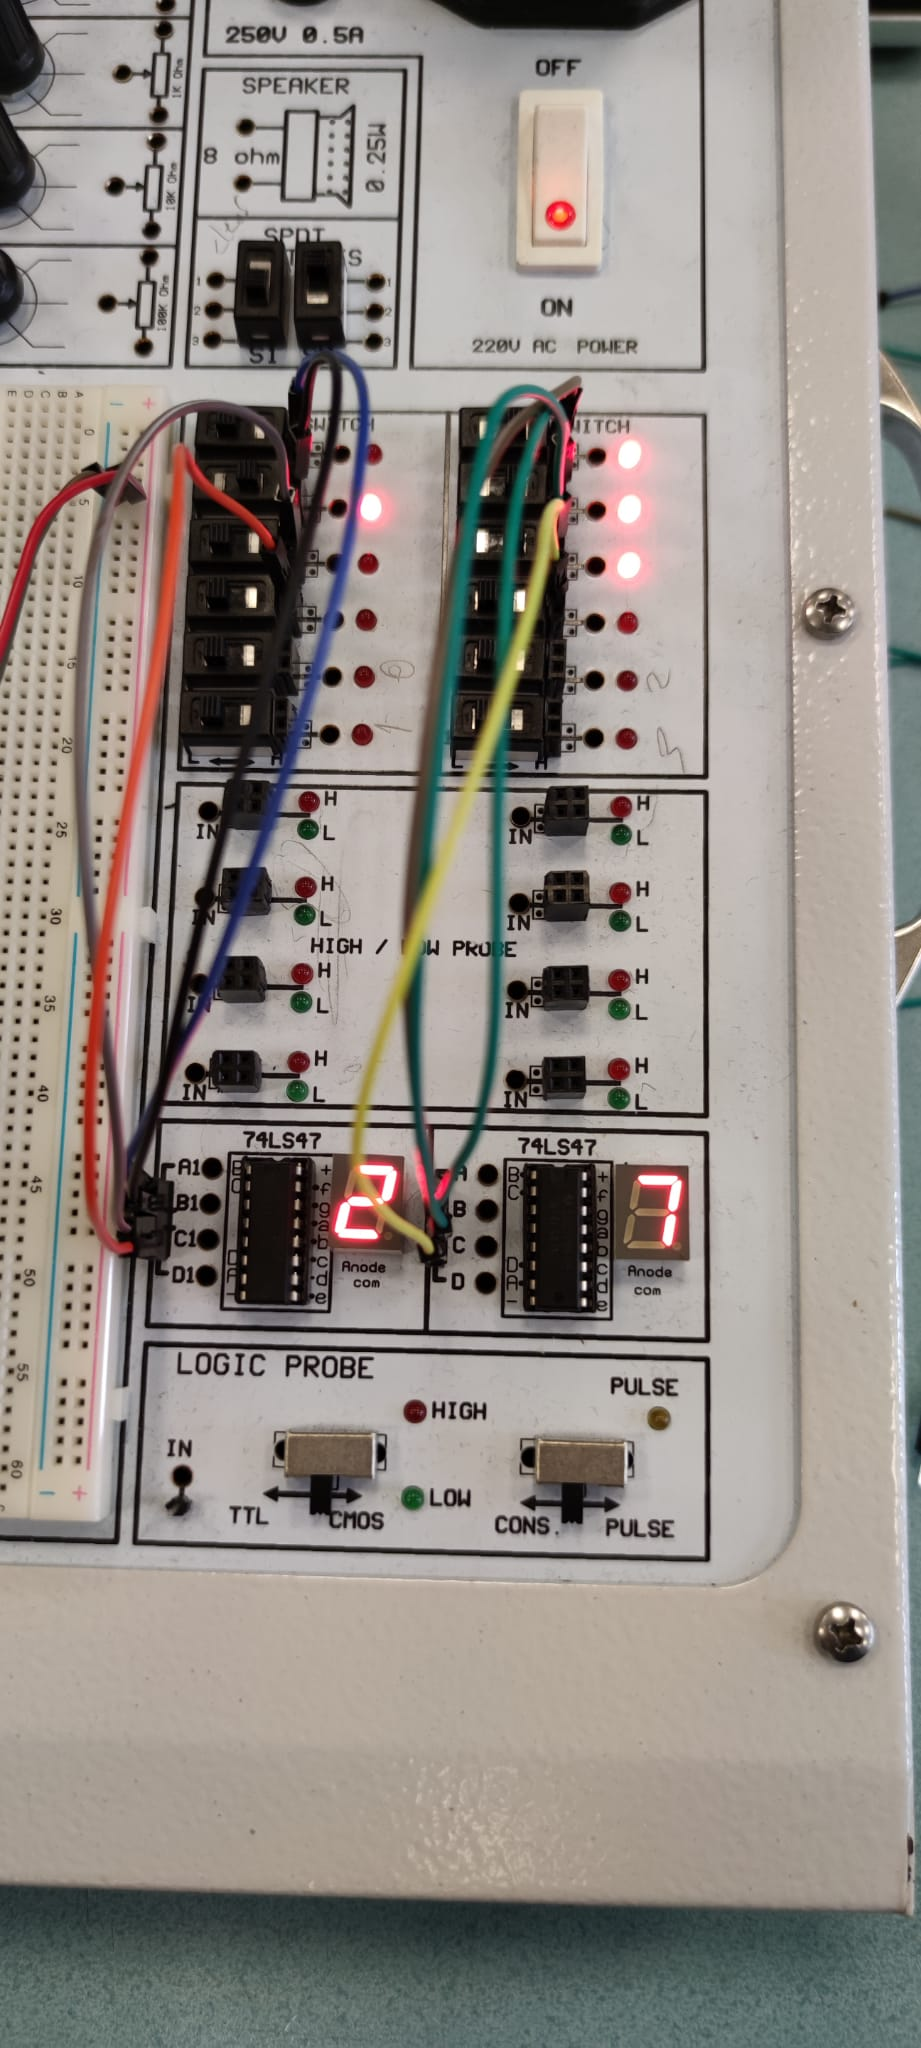
\includegraphics[width=0.5\textwidth]{ex5-3.png}
	\caption{27 on the Seven Segment Display}
	\label{fig7}
\end{figure}

\end{itemize}
\subsection{Part 6}
On this experiment, multiple functions were generated and observed using a oscilloscope.
    \begin{figure}[H]
	\centering
	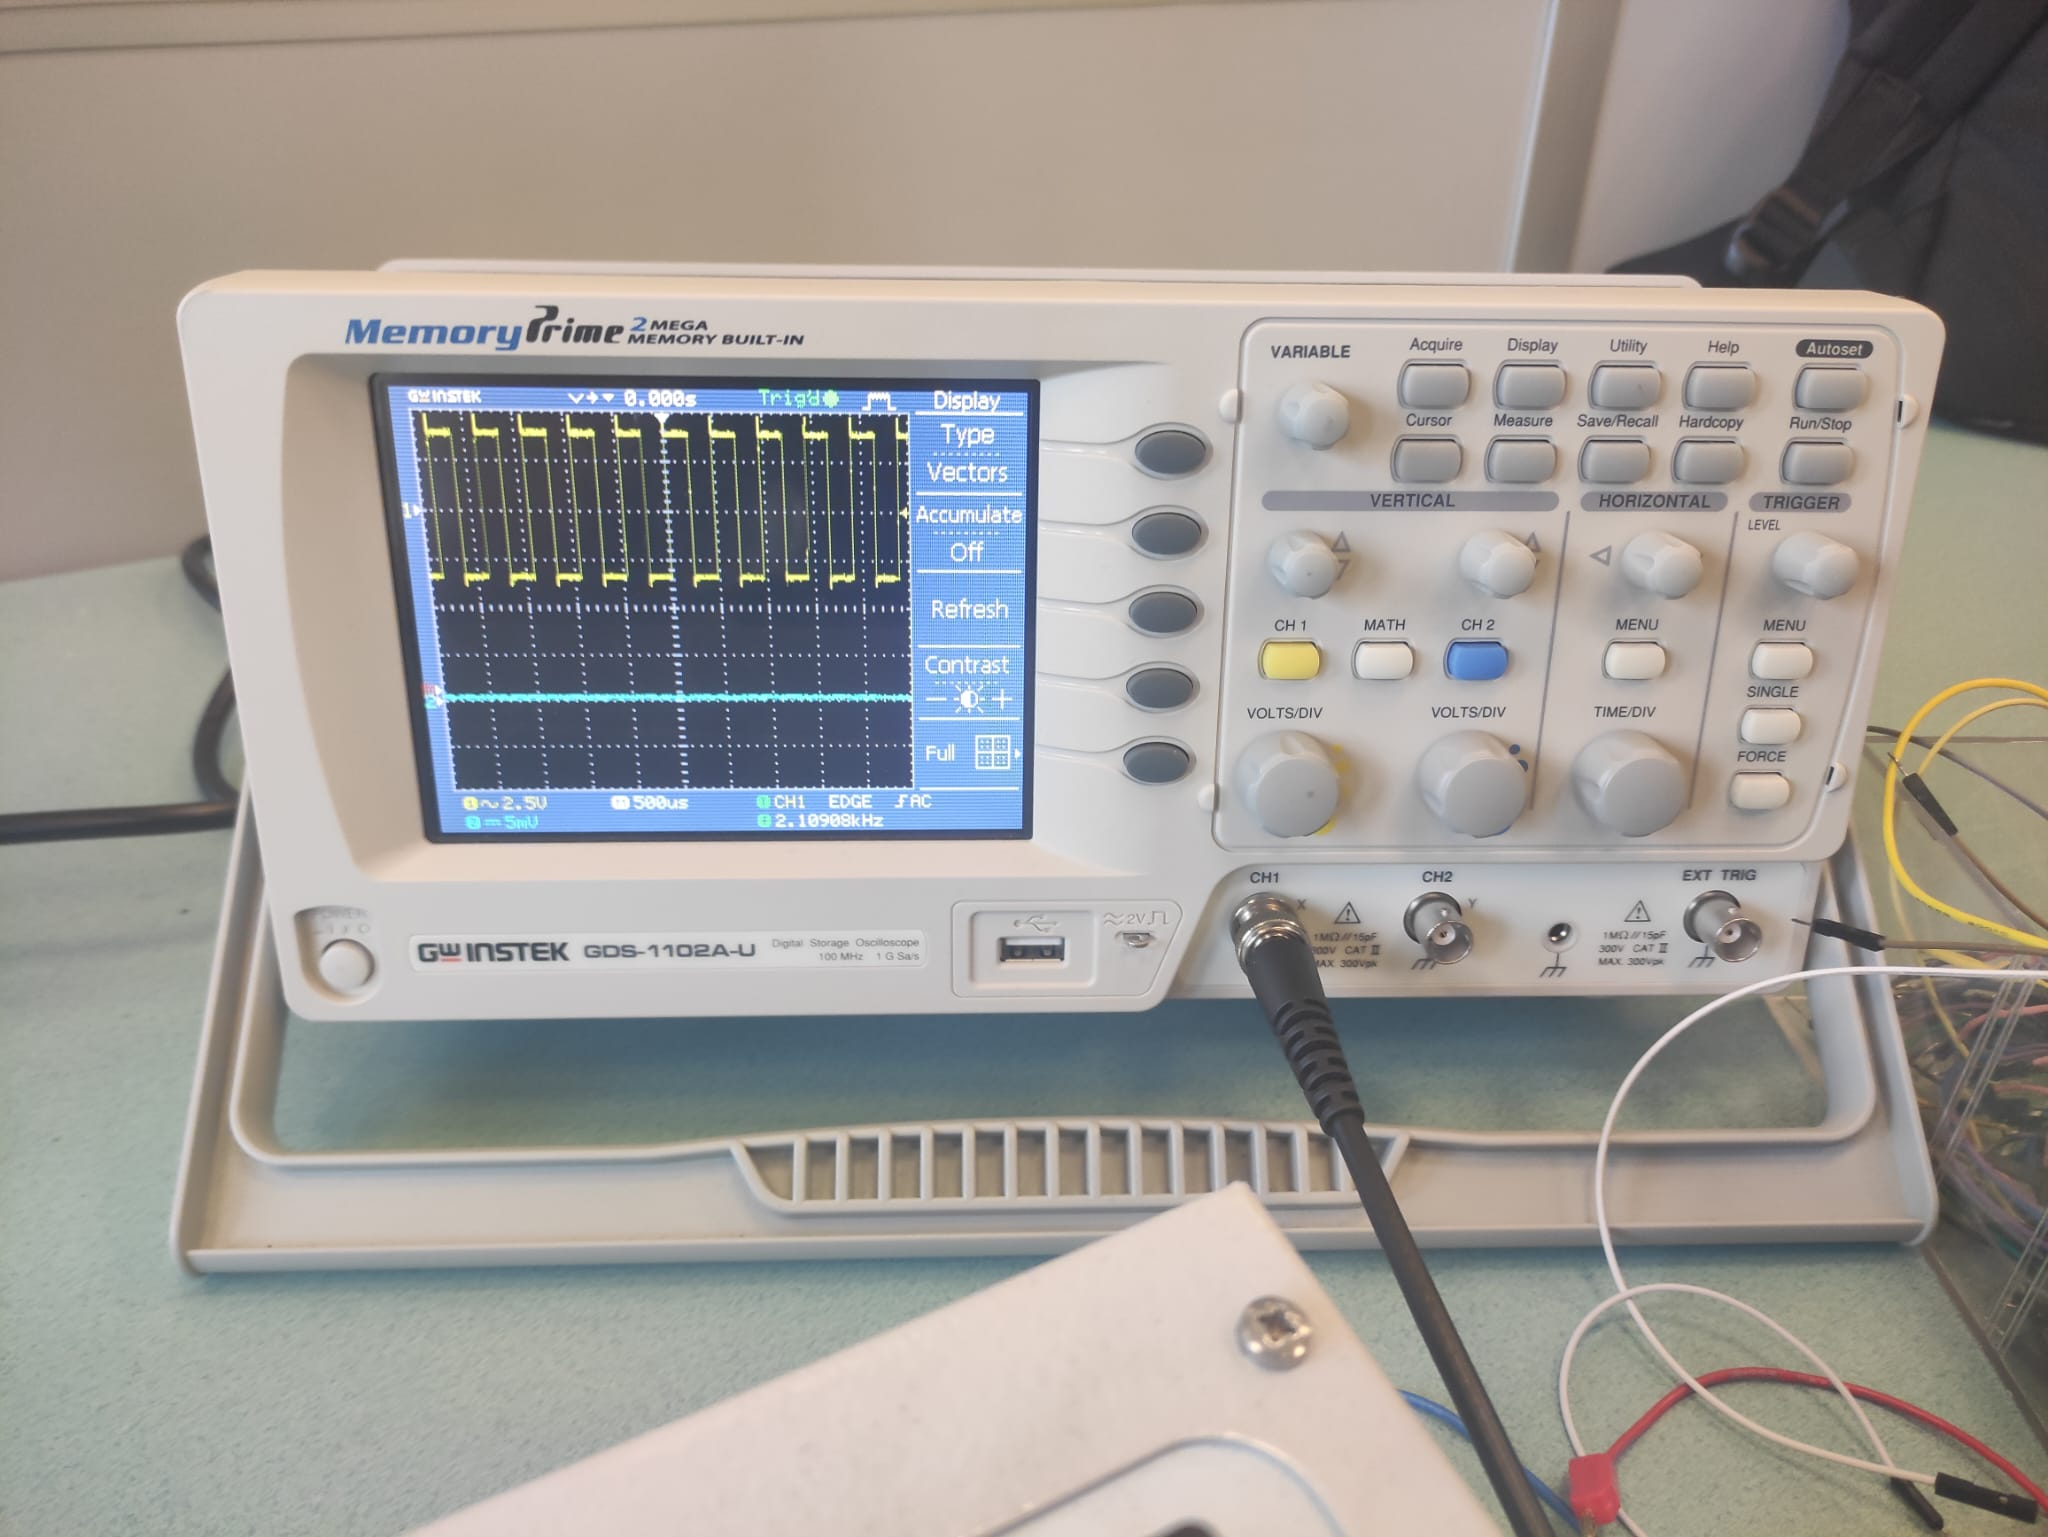
\includegraphics[width=.7\textwidth]{ex6-1.png}
	\caption{}
	\label{fig8}
\end{figure}

\begin{figure}[H]
	\centering
	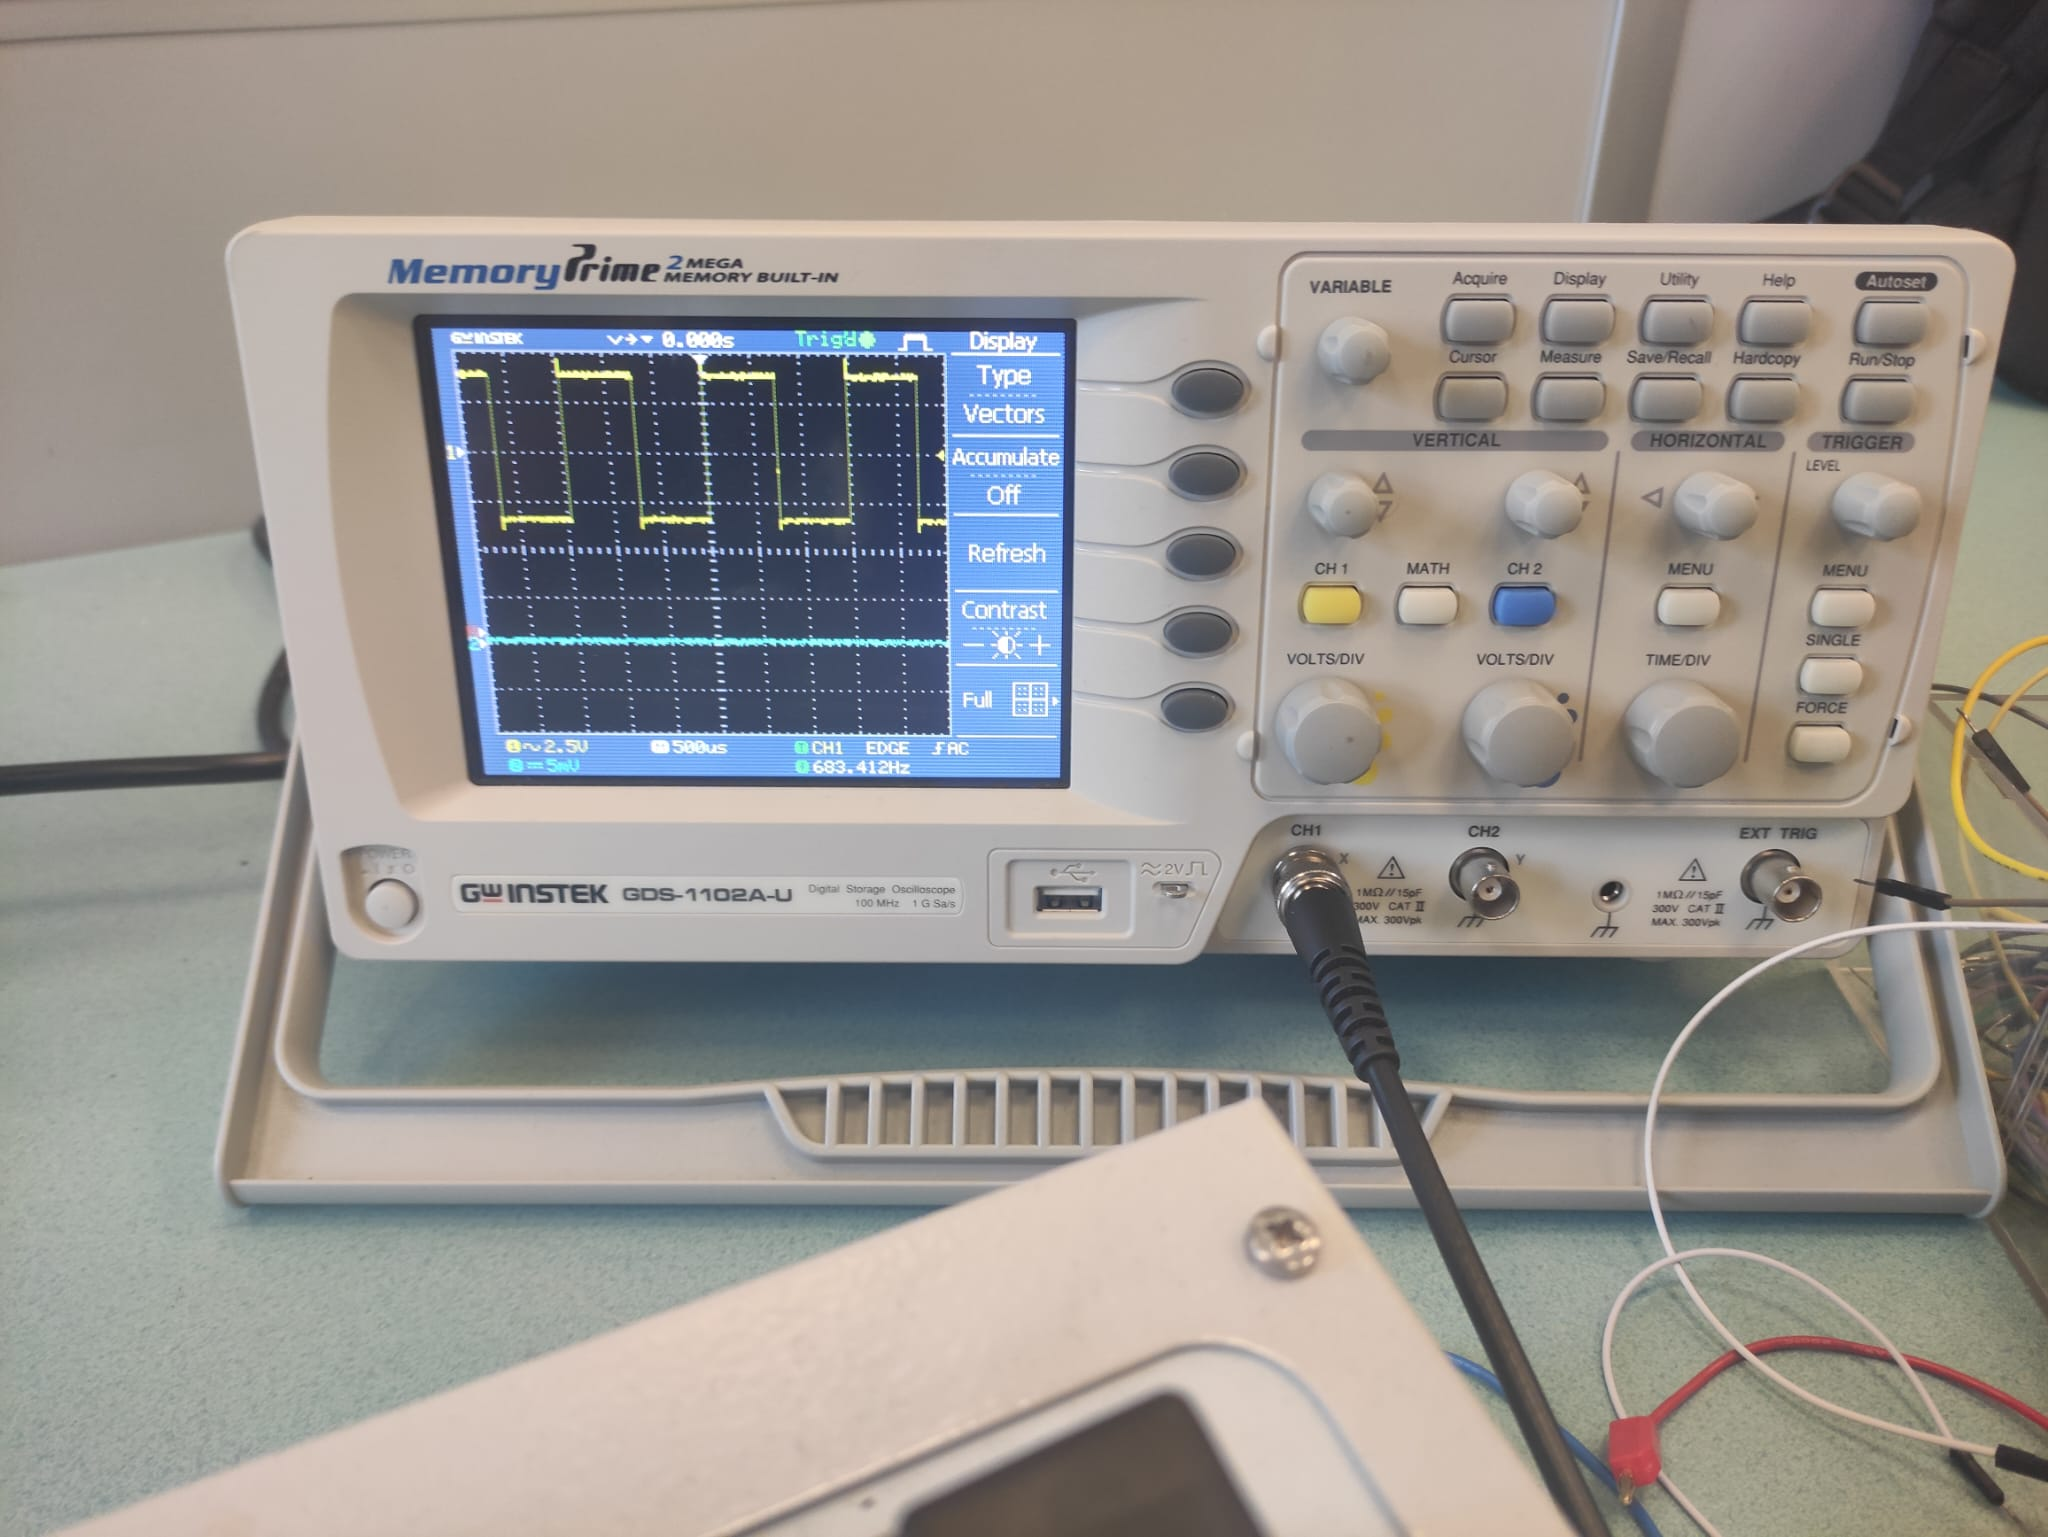
\includegraphics[width=.7\textwidth]{ex6-2.png}
	\caption{}
	\label{fig9}
\end{figure}

\begin{figure}[H]
	\centering
	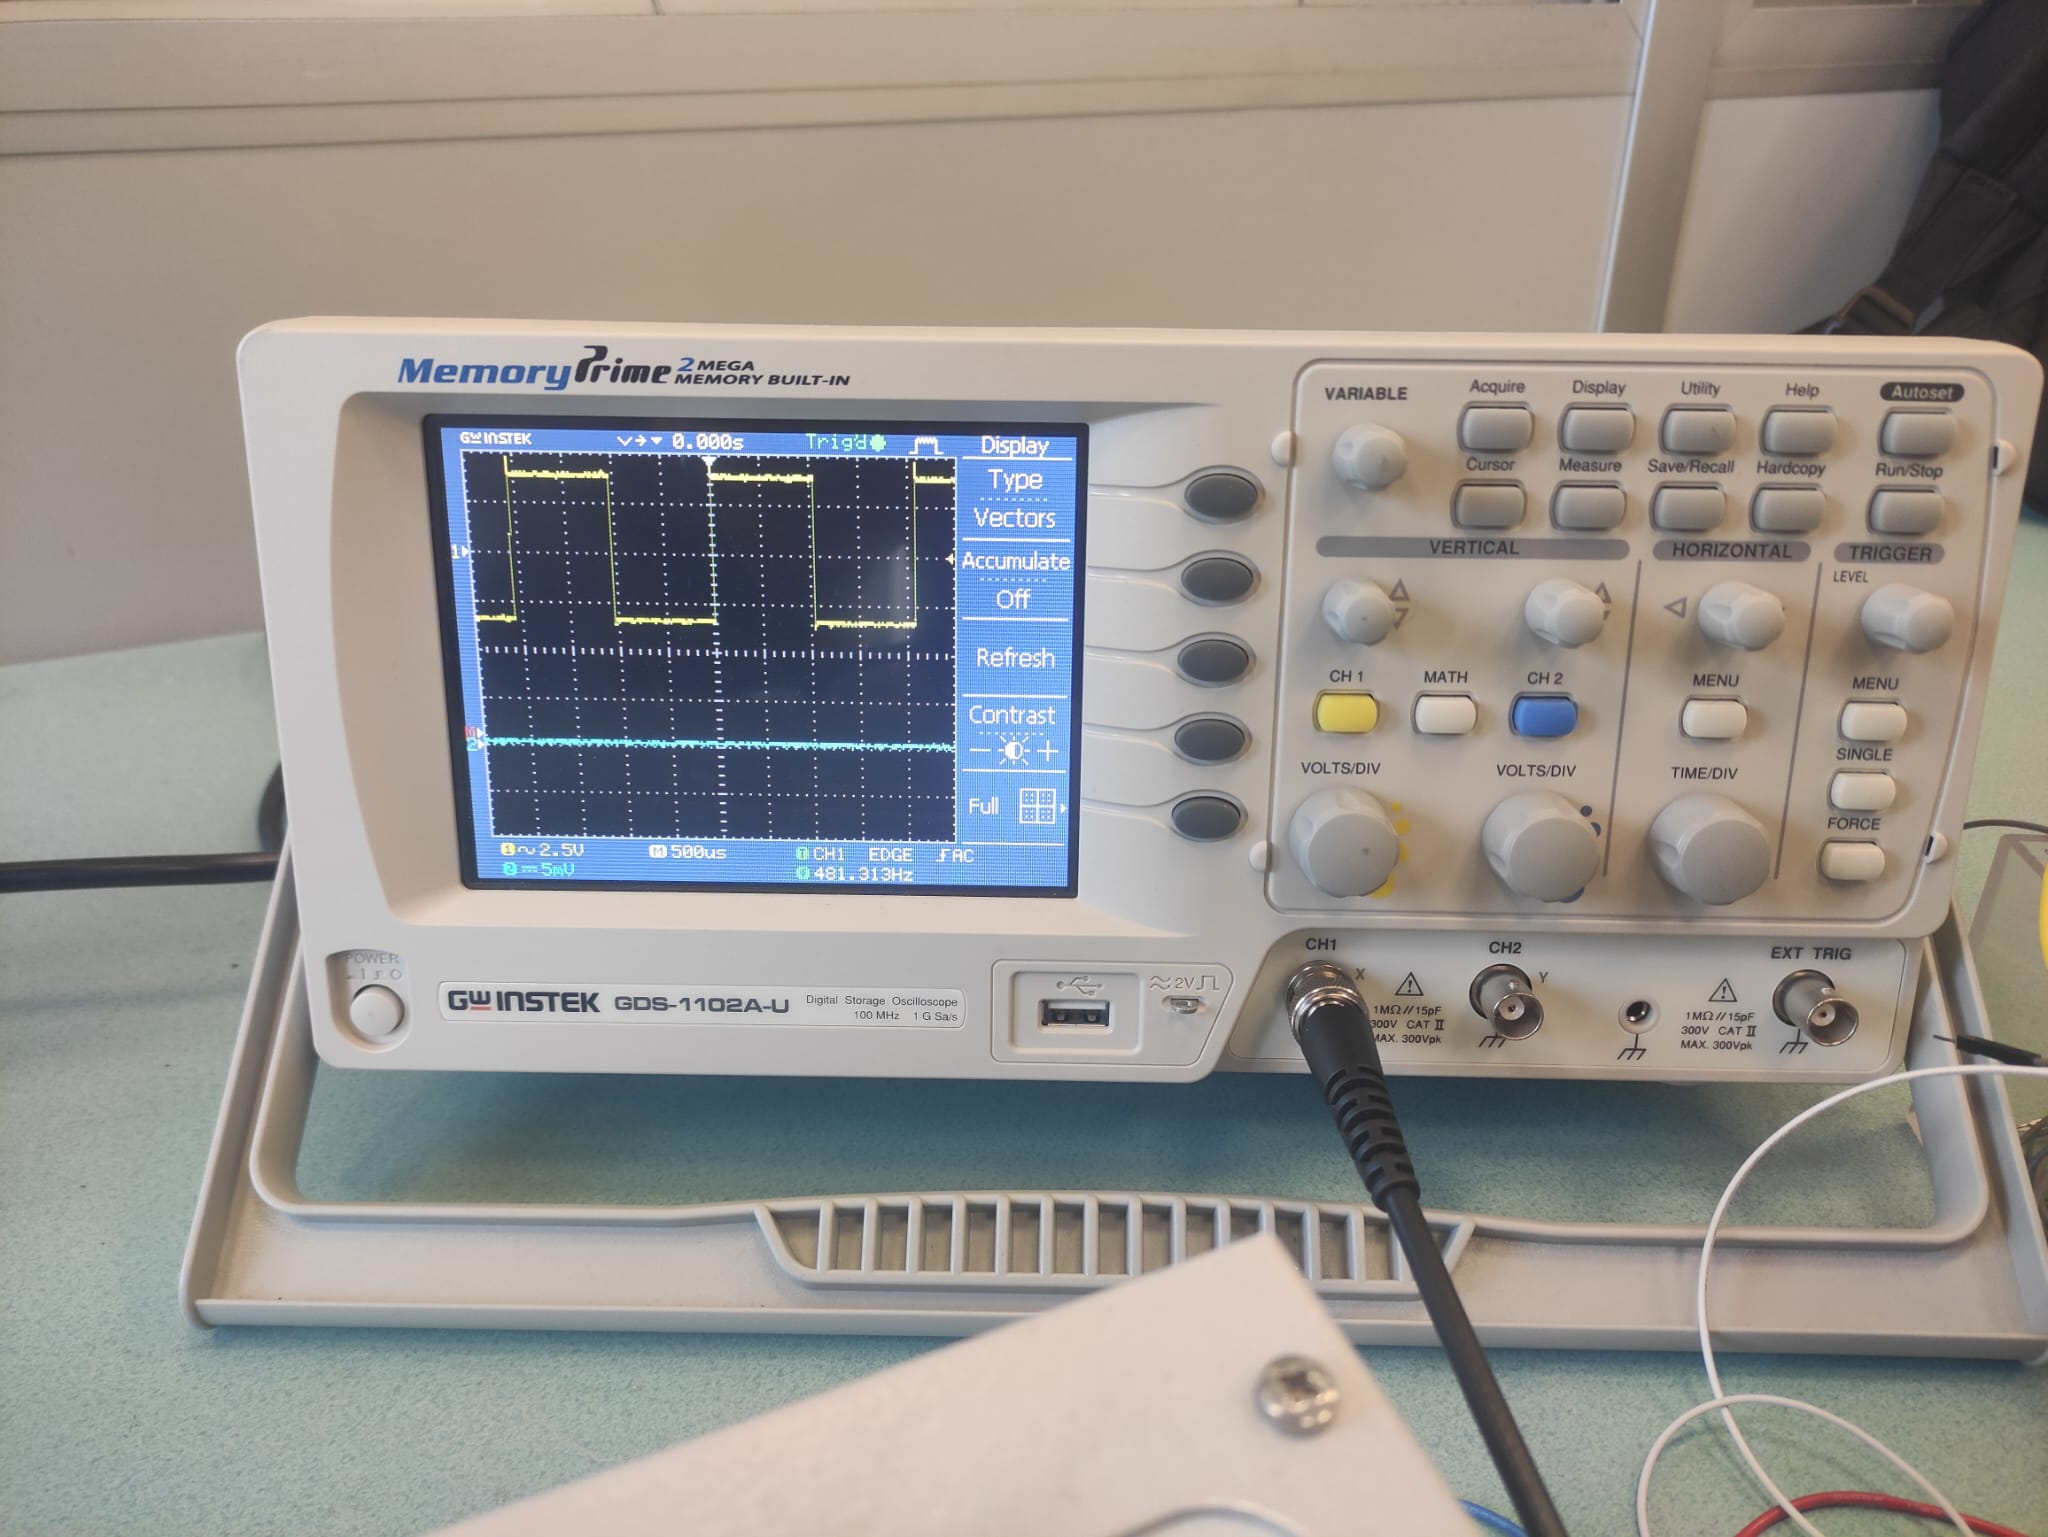
\includegraphics[width=.7\textwidth]{ex6-3.png}
	\caption{}
	\label{fig10}
\end{figure}

\begin{figure}[H]
	\centering
	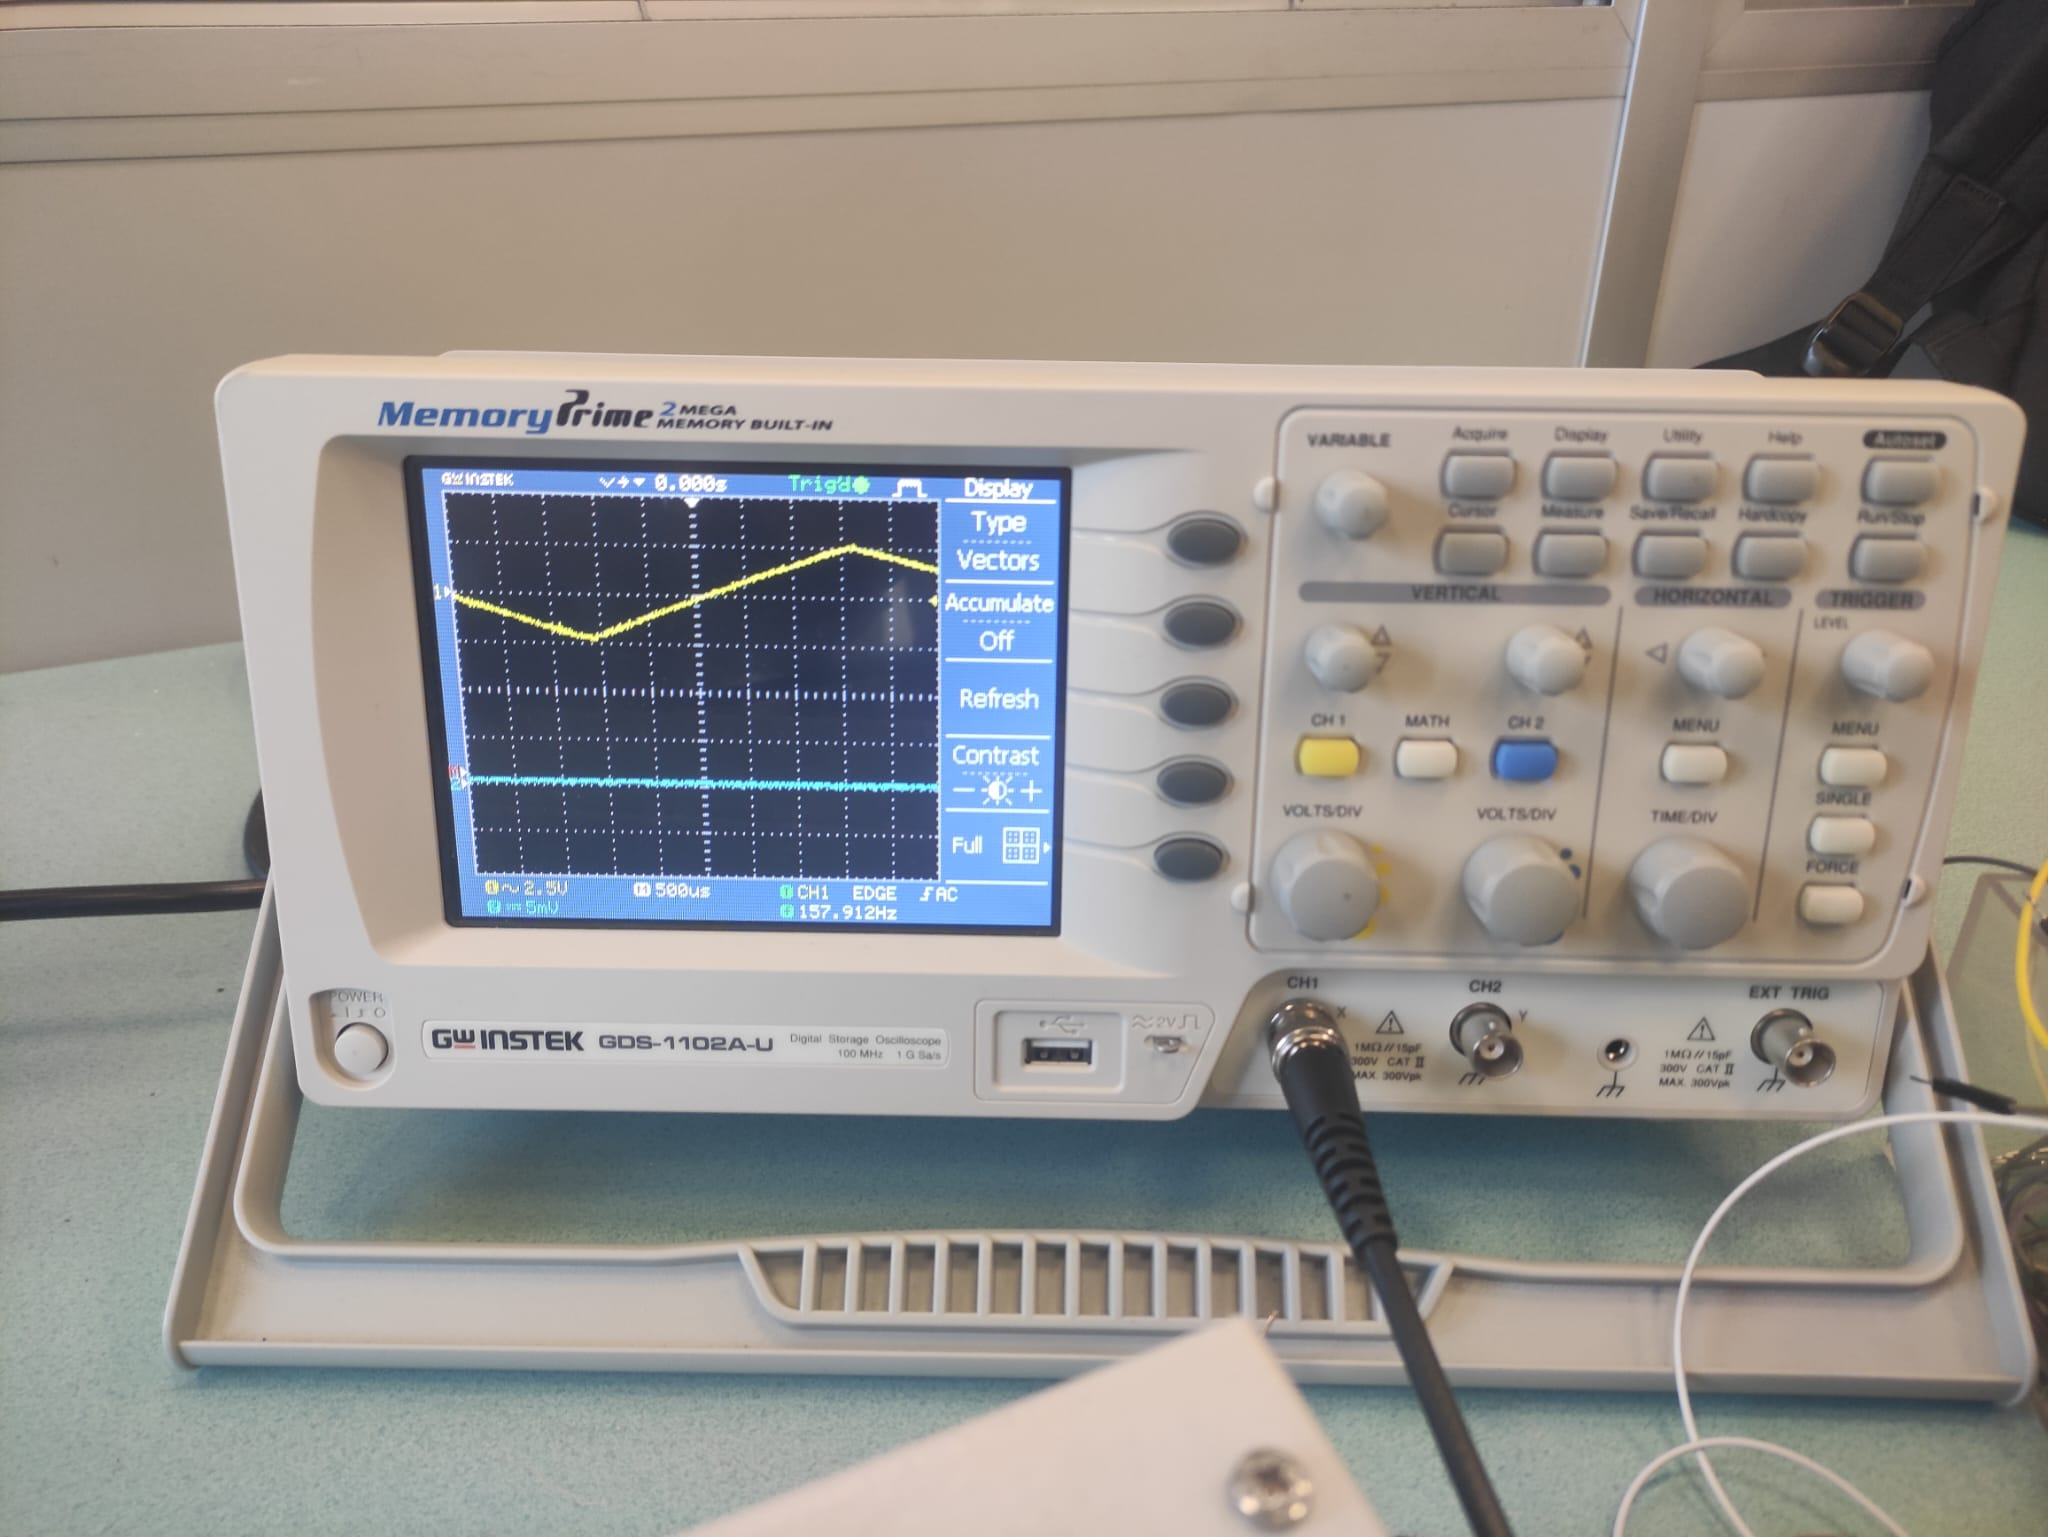
\includegraphics[width=0.7\textwidth]{ex6-4.png}
	\caption{}
	\label{fig11}
\end{figure}

\begin{figure}[H]
	\centering
	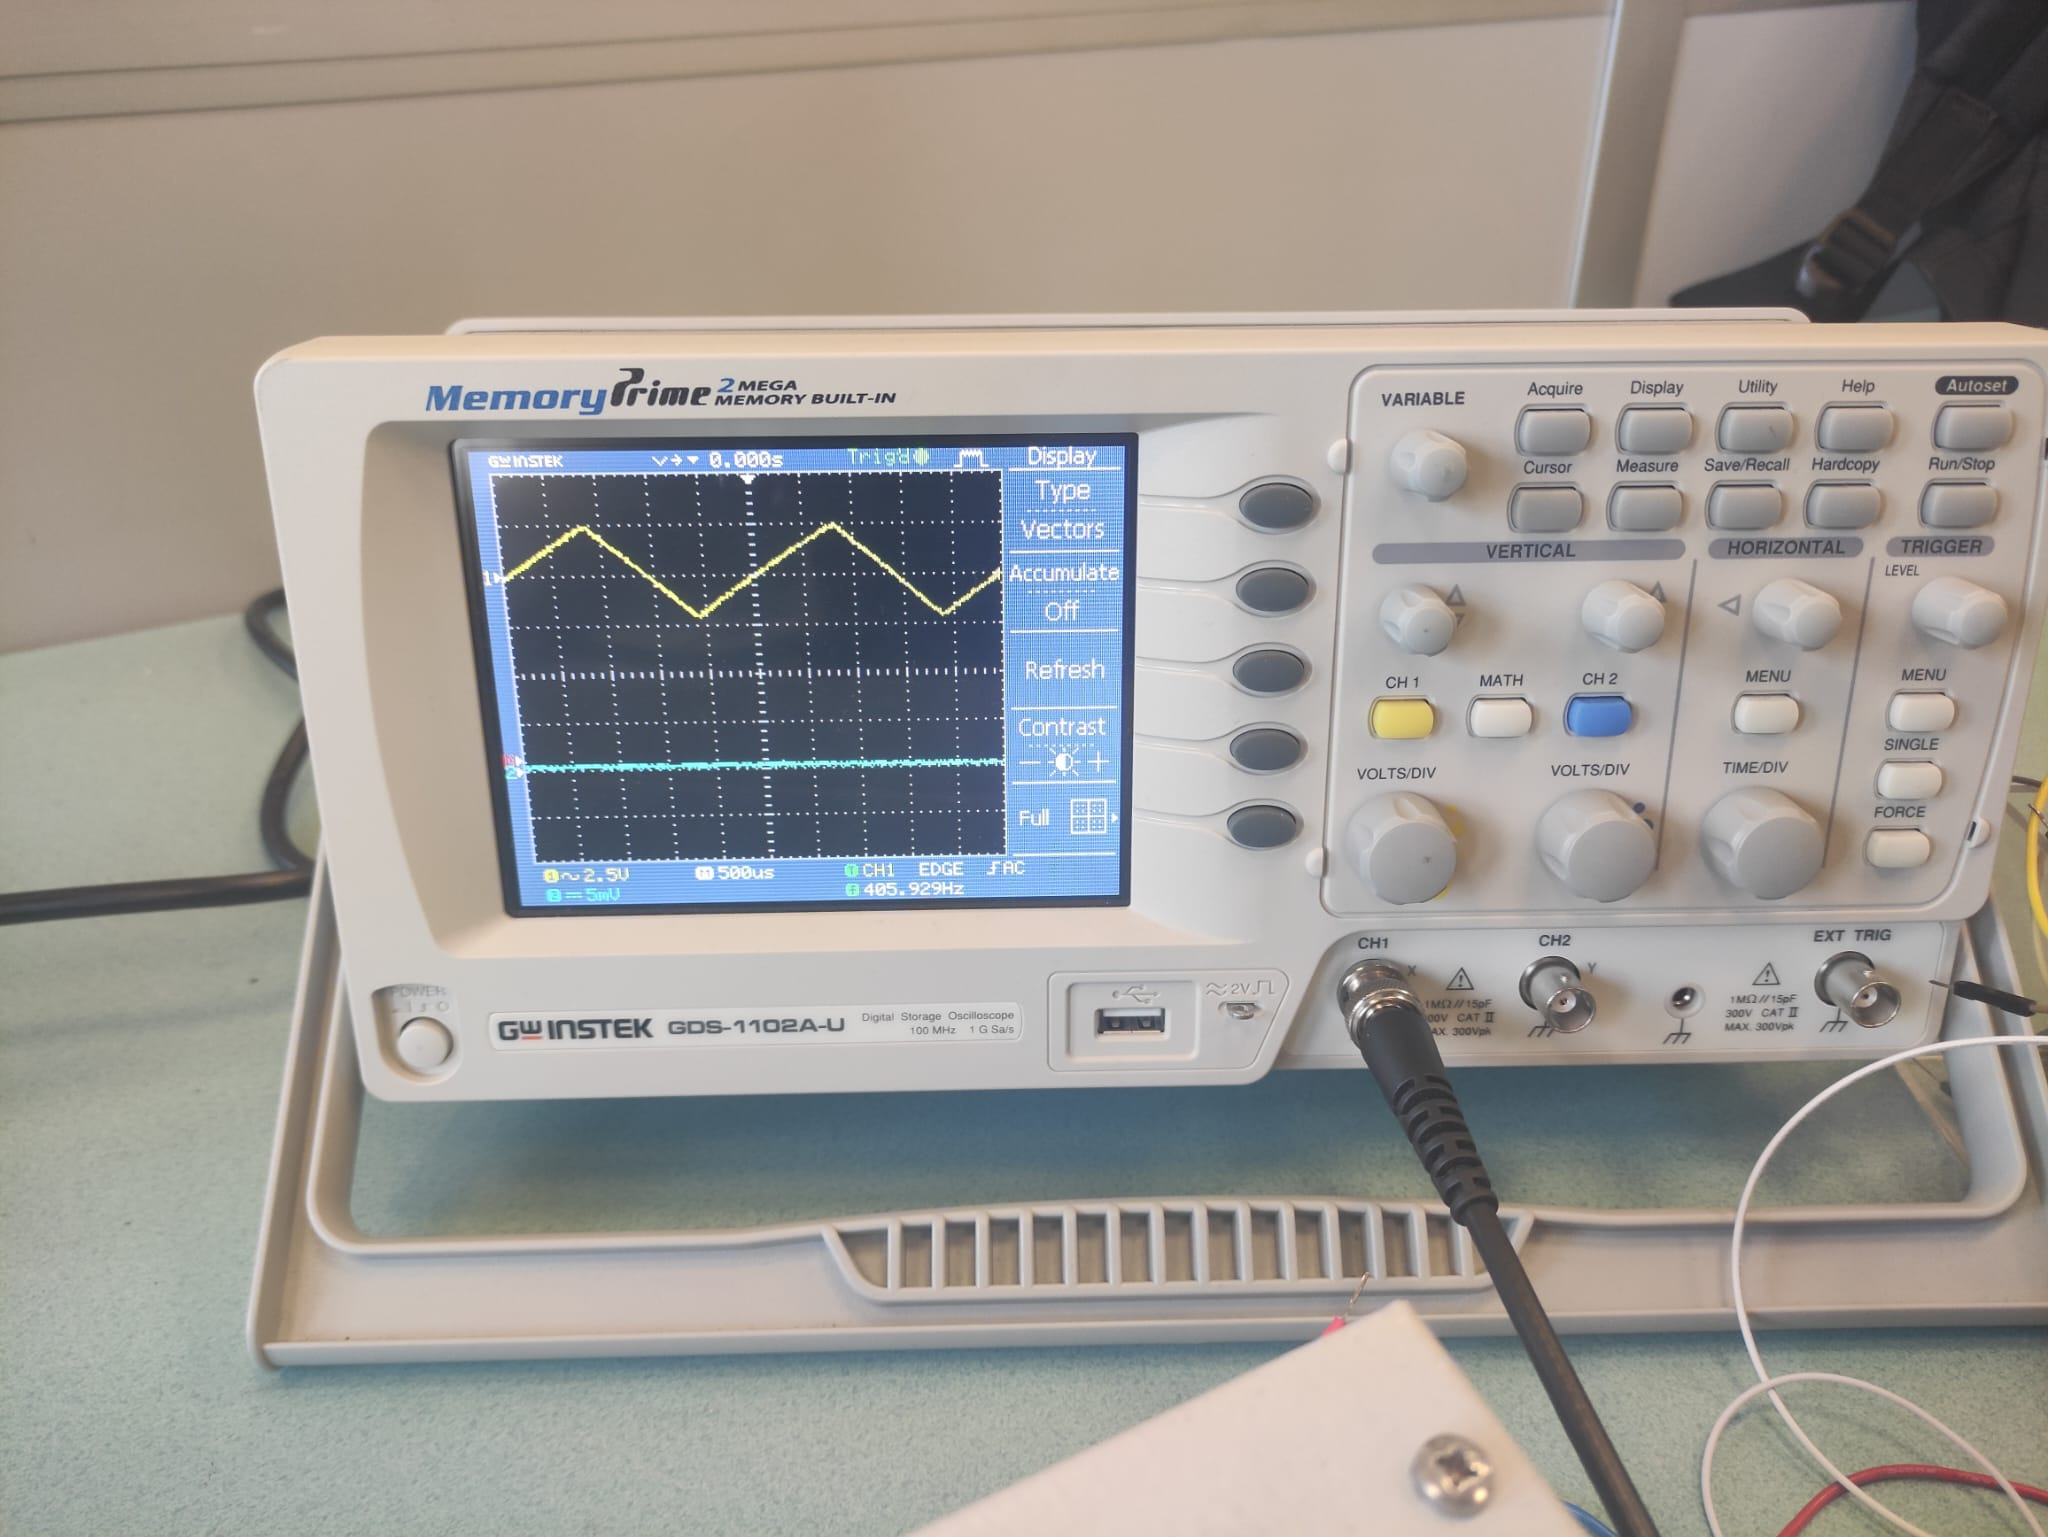
\includegraphics[width=0.7\textwidth]{ex6-5.png}
	\caption{}
	\label{fig12}
\end{figure}

\begin{figure}[H]
	\centering
	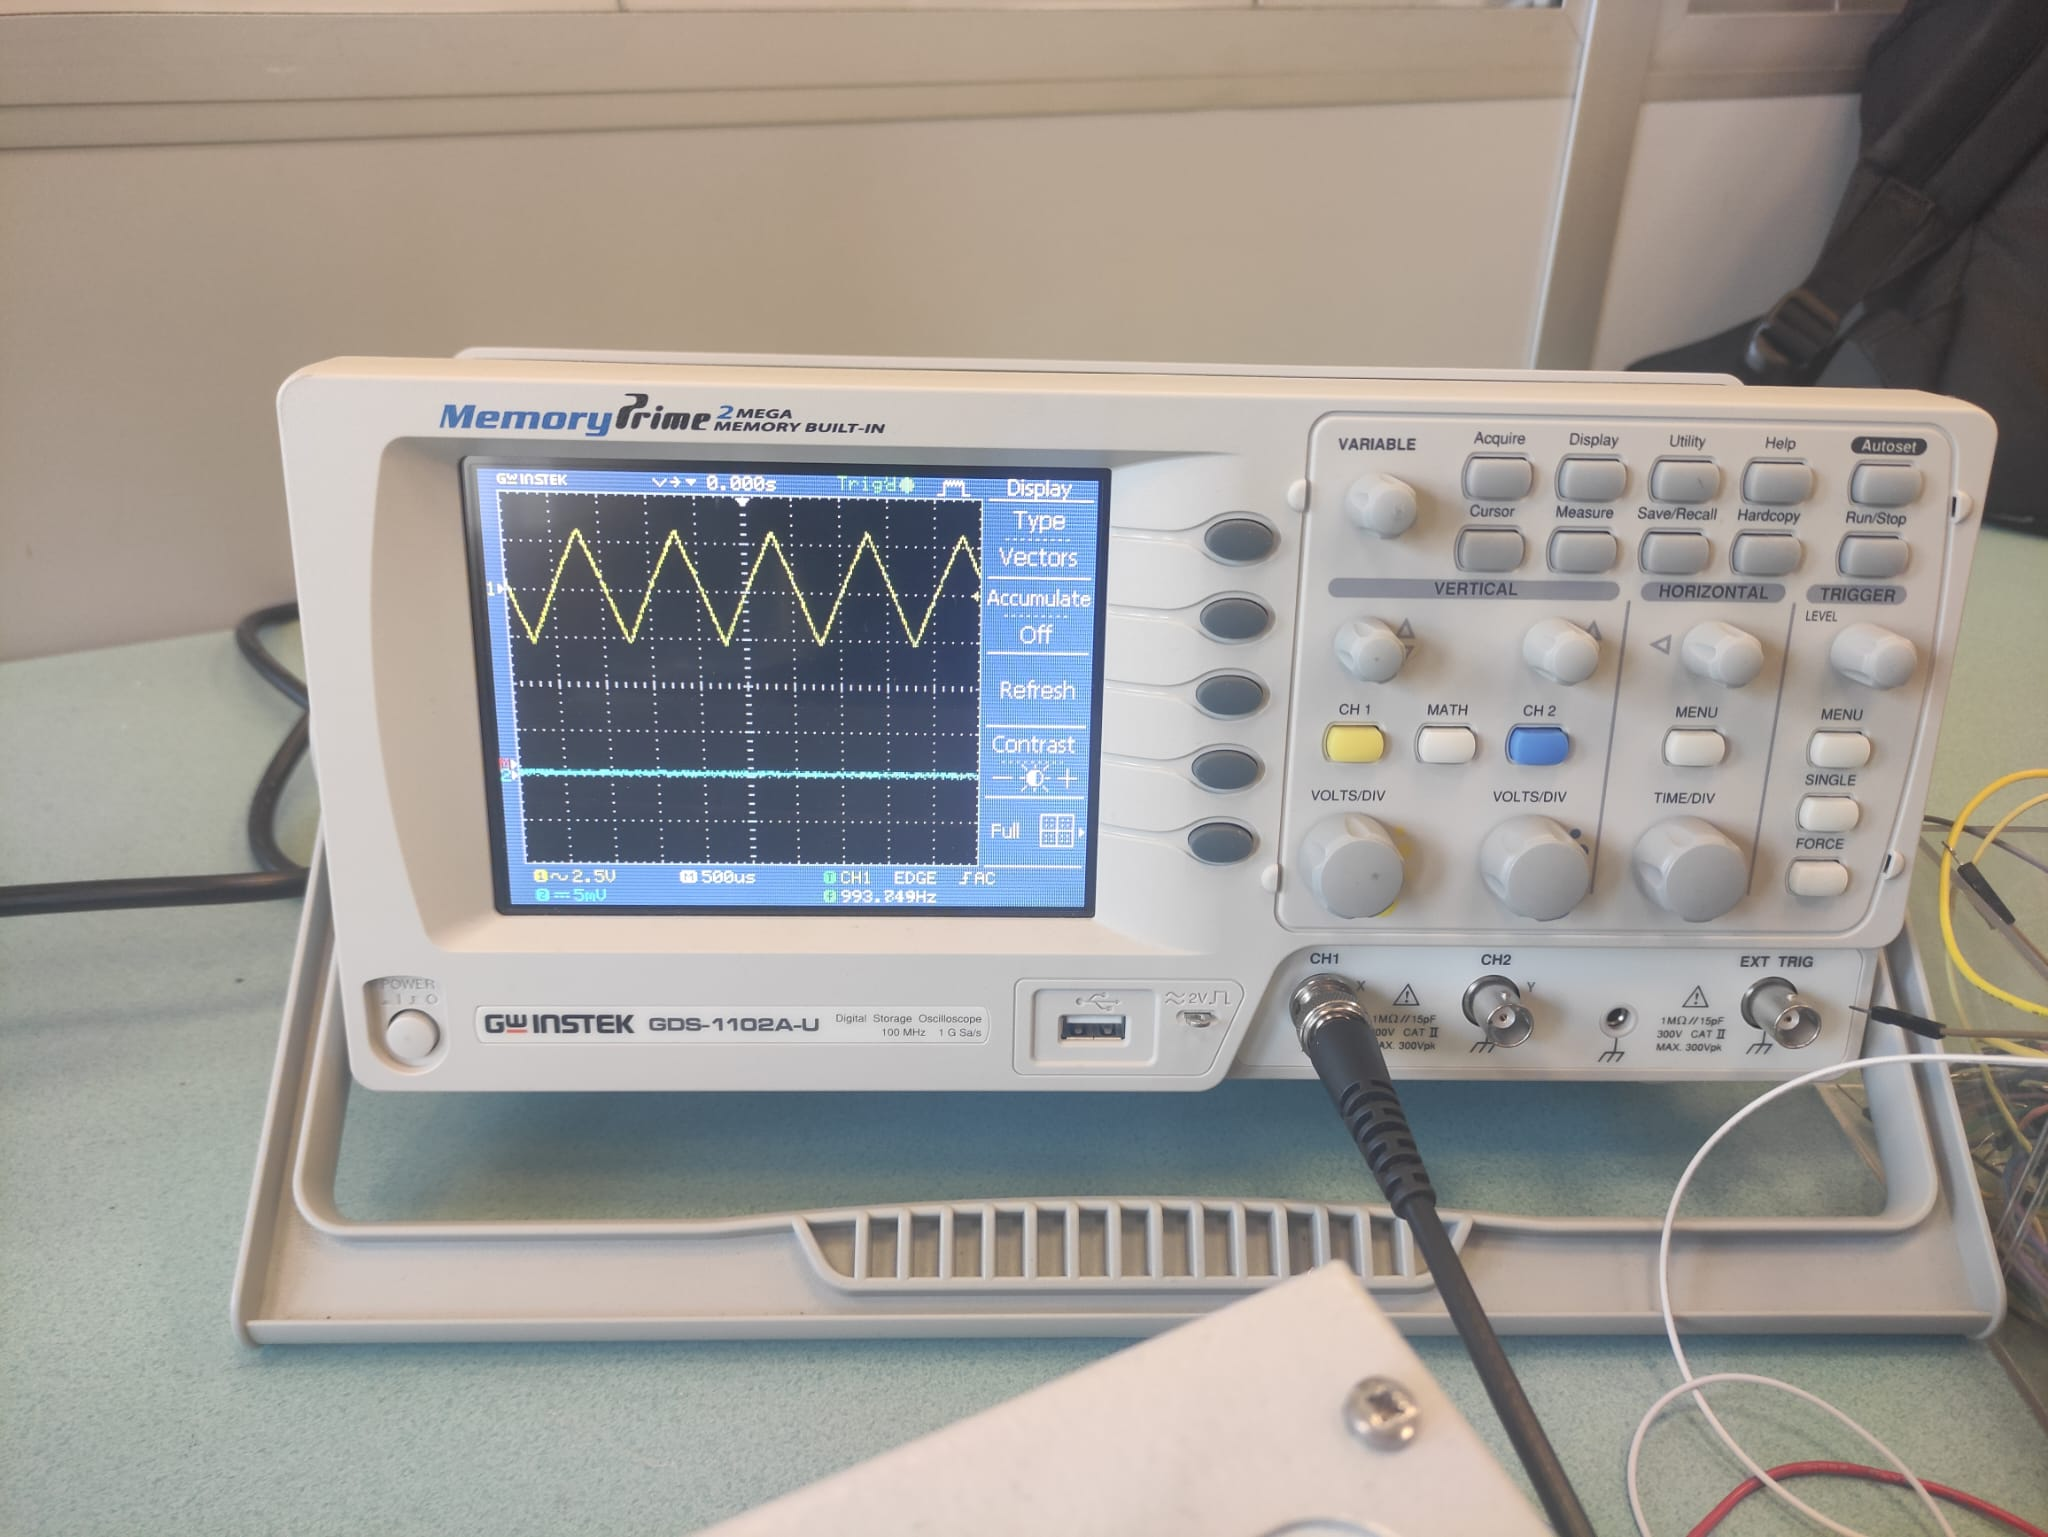
\includegraphics[width=0.7\textwidth]{ex6-6.png}
	\caption{}
	\label{fig13}
\end{figure}

\begin{figure}[H]
	\centering
	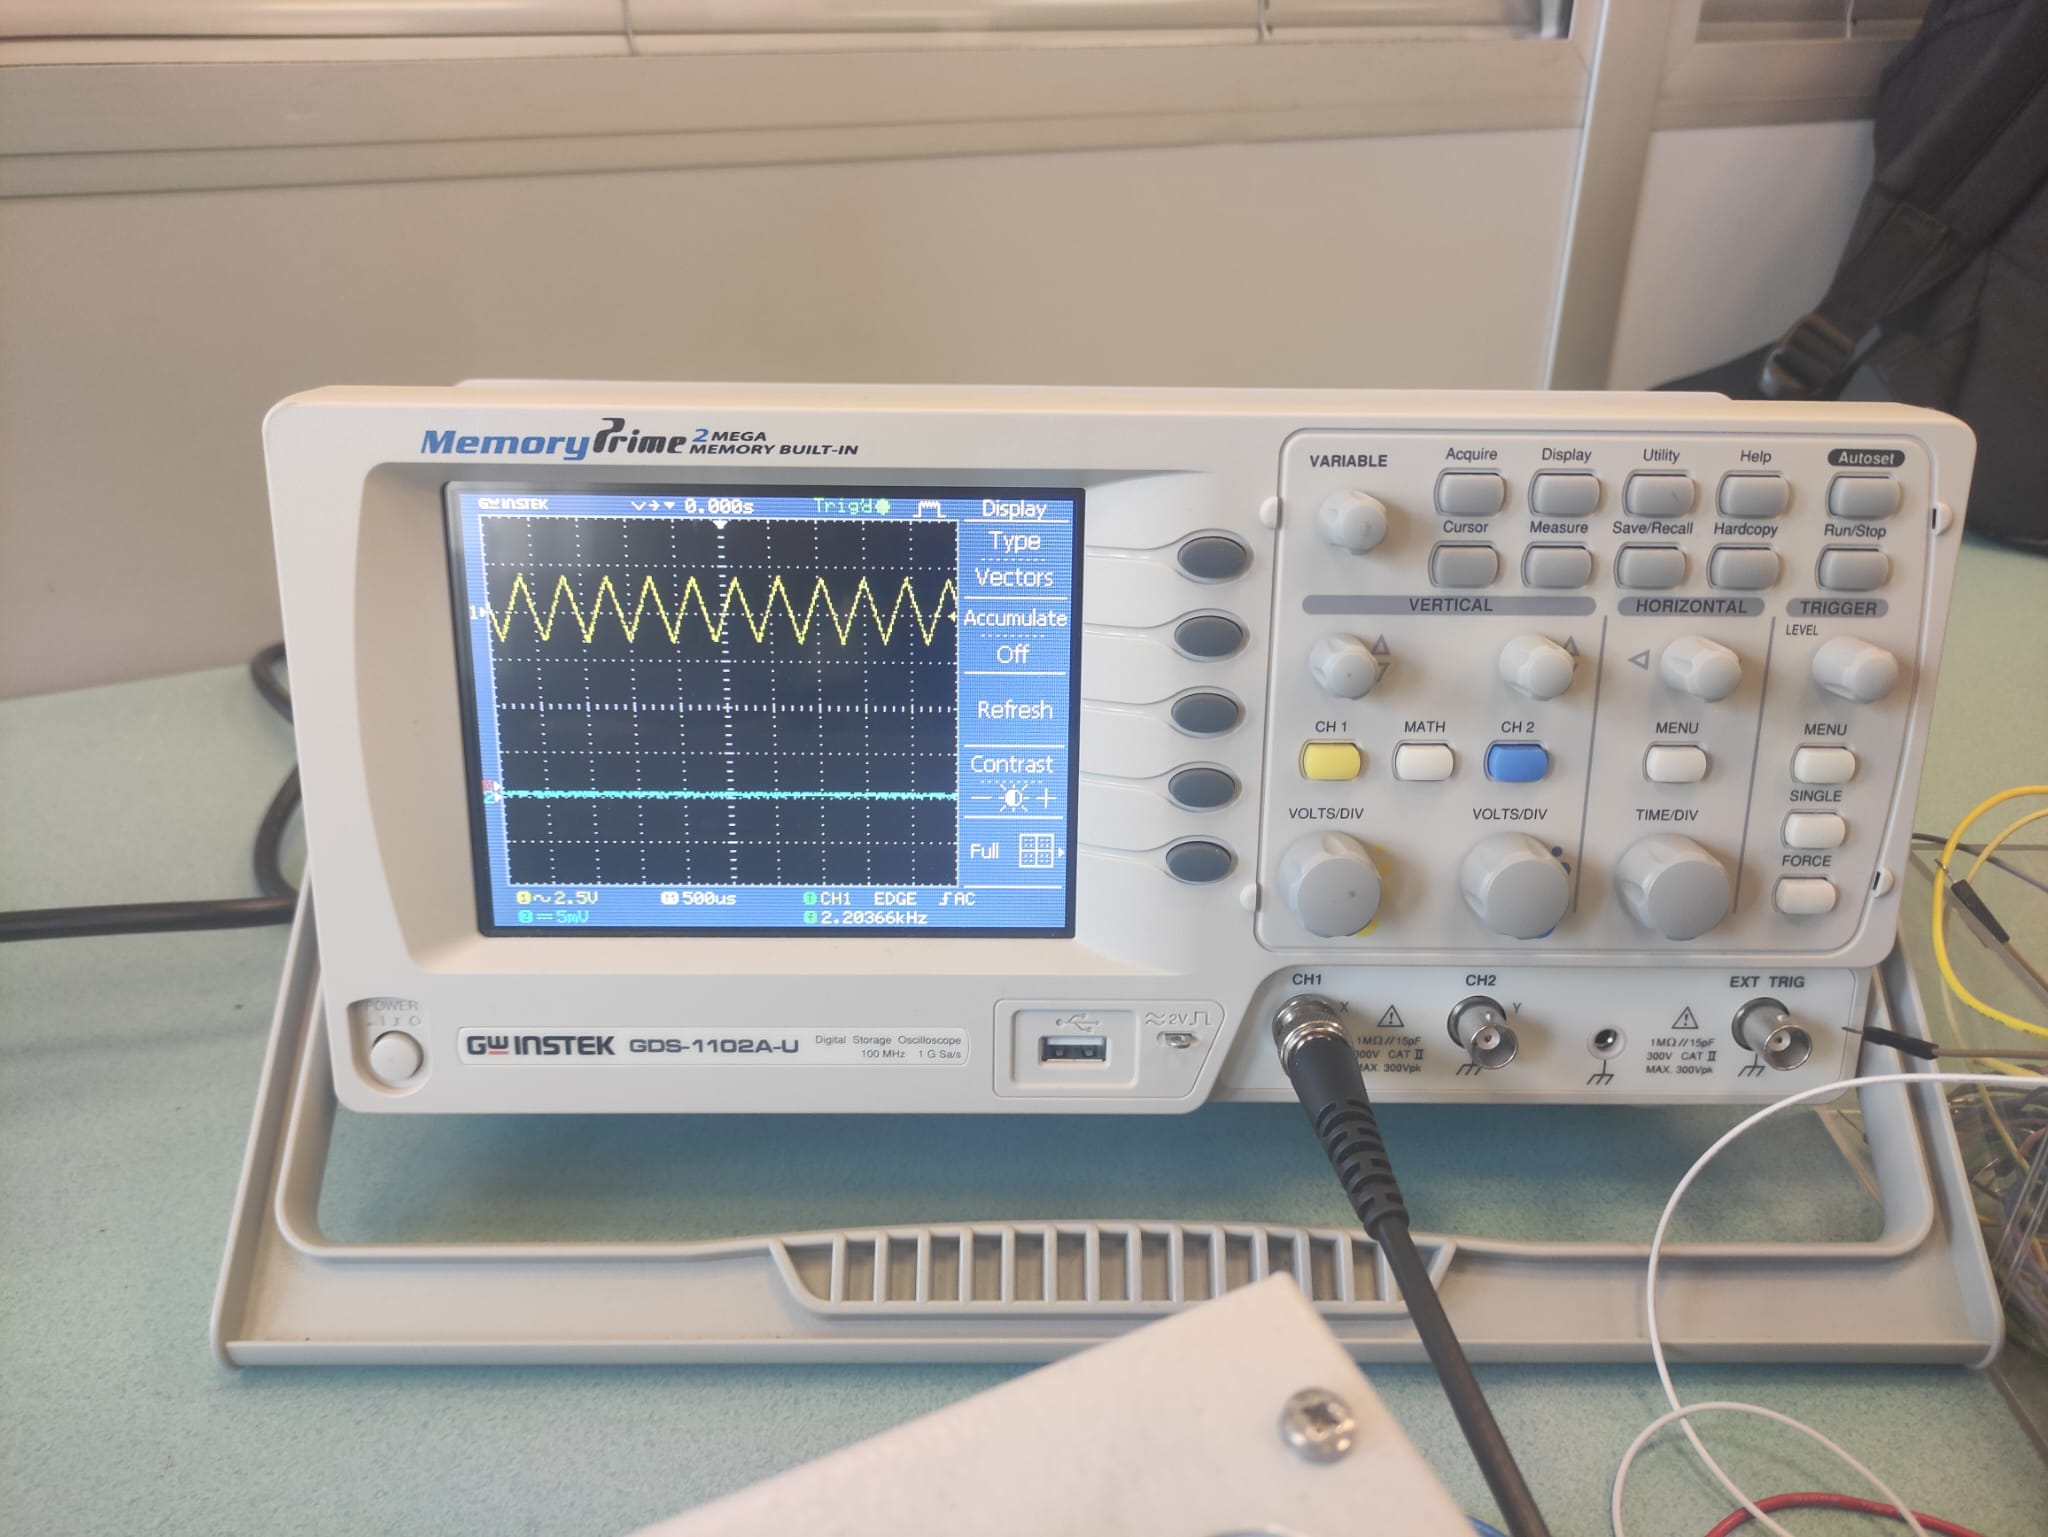
\includegraphics[width=0.7\textwidth]{ex6-7.png}
	\caption{}
	\label{fig14}
\end{figure}

\section{RESULTS [15 points]}
\begin{itemize}
    \item The outcomes of both expressions are the same, as we observed in part 1.
    \item In part 2, it is demonstrated that the theorem's counterpart is logically equal to the theorem itself.
    \item F and its complement always have the opposite truth values, according to the truth table in part 3.
    \item Part 4 makes it clear that the truth value of F is independent of the variables a and b, hence the simplified form does not include them.
    \item In part 5,
    \begin{itemize}
        \item We noticed that the CADET's 5V voltage supply is not exactly determined by a voltmeter to be 5V.
        \item We found that any resistance value, including 8K Ohm, could be attained with little changes.
        \item We discovered that we could modify 7 segment displays in such a way as to display all the numbers, including 27 with the precise combination of inputs.
    \end{itemize}
    \item In part 6, we examined several functions produced by the function generator using the oscilloscope.
\end{itemize}
The numerical findings of the experiments were rather close to what was predicted. We found no appreciable differences between these values. The MATERIALS AND METHODS part of this paper includes pictures of the outcomes of these investigations.

\section{DISCUSSION [25 points]}
We became familiar with the components of CADET while conducting this experiment. We learned how to use integrated circuits on the breadboard of CADET and how to power them correctly. Also, we learned how to use input switches and how to check the output results. With our newfound familiarity with voltmeter, potentiometer and input switches, we learned how to operate seven section displays. We finally understood the fundamentals of the oscilloscope and the function generator.

\section{CONCLUSION [10 points]}
Without too many issues, we completed the experiment from beginning to end. There were simply minor difficulties. For instance, we replaced the faulty part with a new one when one of our integrated circuits on one of the parts was not functioning properly. There were only these two setbacks: we nearly ran out of time and repeatedly forgot to connect a connection to an output indication.

\newpage
\addcontentsline{toc}{section}{\numberline {}REFERENCES}

\bibliographystyle{unsrt}
\bibliography{reference}

\end{document}

